\chapter{Introduction}
\label{introduction}

%\dropcap{E}ver since its introduction in 1983, the Internet has grown to a global communication network used by individuals to interact with others.
%Nowadays, numerous companies operate large-scale digital platforms to facilitate on-line interactions between potentially billions of users.
%eBay was one of the first platforms that enabled the trustworthy trade of goods between merchants and buyers over the Internet, and is used by millions on a daily basis.
%More recently, companies acting in the sharing economy, like Uber and AirBnb, shaped the notion of digital interactions between individuals over the Internet.
%These companies facilitate peer-to-peer resource sharing where strangers can share personal resources, like their house or car, in a trustworthy manner.

%Most of the on-line applications we use on a daily basis are \emph{centralized}, e.g., managed by a single authority that maintains the required network infrastructure. % facilitated by centralized architectures, often deployed and maintained by a single company.
%In particular, when considering a centralized Internet application, there is a single or limited group of servers, responsible for processing all requests submitted by the platform participants, e.g., uploading a video on YouTube or posting a tweet on Twitter.
%Hosting the network infrastructure to facilitate interactions on a global scale requires major investments and platform costs, as exemplified by major companies like Facebook and Google.
%On one hand, centralized infrastructures are relatively easy to setup and their performance can be increased by deploying more servers.
%On the other hand, even a single software bug or hardware failure could lead to a prolonged unavailability of the entire application.
%For example, Facebook experienced a day of downtime in March 2019 due to a server misconfiguration.

%In comparison, \emph{decentralized} applications aim to avoid reliance on a single authority.
%A decentralized application consists of a network where computers directly communicate and collaborate with each other instead.
%One of the most popular decentralized applications is the BitTorrent file transfer protocol, used to share and download torrent files.
%In BitTorrent, users directly exchange parts a (potentially large) file with each other over the network, without any requirement for servers that are under the control of a single authority.
%Although the global unavailability of a decentralized application is a rare phenomena, they often are more vulnerable to attacks targeted at the network layer, such as the Sybil Attack and the Eclipse Attack.

\dropcap{A} marketplace facilitates the exchange of services, goods and information between individuals and businesses~\cite{bakos1998emerging}.
Marketplaces play an important role in our economy, enabling the exchange of value on a massive scale.
Electronic commerce, or \emph{e-commerce}, makes up a large part of global conducted trade.
A recent report estimates that e-commerce entails \$800 billion (the bottom-up estimate) to \$1.5 trillion (the top-down estimate)~\cite{ecommerceestimate}.
%The Internet provides the infrastructure to globally exchange information and to deploy large-scale electronic marketplaces, e.g., Amazon and eBay.
Large-scale electronic marketplaces like Amazon and eBay have long dominated the field of e-commerce.
During the last decades, however, companies acting in the \emph{sharing economy} (e.g., Uber and AirBnb) have expanded the notion of e-commerce by offering global marketplaces for the sharing of personal resources (e.g., cars and houses) with strangers.\footnote{This is also known as \enquote{stranger sharing}~\cite{schor2016debating}.}
%On electronic markets, traders routinely trade with other traders with whom they never interacted before, unlike in many physical marketplaces.
%During the last decade, this effect has been amplified by companies acting in the \emph{sharing economy}, like Uber and AirBnb.
%The notion of sharing personal resources with strangers (e.g., cars and houses) has long been perceived as unreliable.

%In general, the role of marketplaces, electronic and otherwise, is three-fold~\cite{bakos1998emerging}.  % https://dl.acm.org/doi/pdf/10.1145/280324.280330
%First, they have to match buyers and sellers, either through an automated matchmaking process or by offering the required functionality for users to browse through the services or goods offered on the market.
%Second, the market has to facilitate transactions, including the delivery of goods from a seller to a buyer and associated payment flows.
%Third, the market has to provide institutional infrastructure for fraud management, dispute resolution and regulatory compliance.

The standard approach to devise electronic marketplaces is by deploying centralized infrastructure, fully operated and managed by a market operator.
This market operator provides the required primitives for bringing buyers and sellers together, for the management of market information (e.g., product listings), and for transaction processing (e.g., by providing payment services).
In addition, the market operator can acts as trusted intermediary between buyers and sellers, leveraging its intermediate position to alleviate or address potential conflicts arising between traders.
For example, the ride-hailing company Uber ensures that its drivers are sufficiently qualified to offer their services to passengers, and process all payments made by passengers.
Market intermediaries usually charge users for their services through transaction fees.

Advancements in information technology, in particular blockchain technology, have challenged the need for both authoritative market operators and trusted intermediaries.
The Bitcoin currency, powered by a tamper-proof distributed ledger, has demonstrated that it is possible to build a cash system not under the ownership of a financial institution~\cite{nakamoto2008bitcoin}.
Similarly, Ethereum enables developers to write legally-binding contractual logic without notaries~\cite{wood2014ethereum}.
The notion of \emph{disintermediation}, removing trusted intermediaries, is closely related to the process of \emph{decentralization} where authority residing in a single entity is re-distributed over multiple entities.
There is an increasing amount of research effort to disintermediate existing platforms with decentralized solutions such as distributed ledgers.
These platforms includes electronic marketplaces.

This thesis orients around decentralization and disintermediation in blockchain-based electronic marketplaces.
A key characteristic of blockchain-based marketplaces is that economic activity emerges from the direct interactions between sellers with minimal involvement of trusted intermediaries.
In this work, we design, implement, evaluate and deploy five decentralized mechanisms that improve different aspects of electronic marketplaces.
These aspects include the storage and dissemination of market knowledge, matchmaking between buyers and sellers, and settlement.
In the remainder of this introduction, we elaborate on the concept of decentralization and disintermediation, and outline blockchain-based marketplaces from a technical perspective.
%While the discussed mechanisms in this thesis focus on different aspects of marketplaces, their common goal is to identify the role of trusted intermediaries and assess if theyr . 
%The remainder of this introduction is structured as follows:, we first outline the impact of the Internet as infrastructure to conduct trade.
%Next, we show how blockchain technology makes it possible to devise marketplaces without middleman.
%Then, we discuss the critical components of blockchain-based marketplaces and present existing approaches to realise each component.
%Finally, we state the main research question that this thesis answers.

\section{Decentralization in Markets}
The term \emph{decentralization} is defined by Merrian-Webster as \enquote{the dispersion or distribution of functions and powers}.
It describe the process by which decision making is delegated away from a central, authoritative entity.
Decentralization is widely used as a term within different branches of science, including economics, social sciences and computer science.
Arguably, the most well-known type of decentralization is \emph{political decentralization} where the authority of national governments regarding policymaking is reduced, e.g., by delegating authority to provinces or municipalities.

In computer science literature, the term \emph{decentralization} is increasingly being used to indicate systems where decisions are not taken by a single entity and where the authority is spread over participants.
This is also how the term decentralization is used throughout this thesis.
Decentralization is usually accredited as a desirable property of a system, raising the bar to manipulate and take down the system since there is not single point of failure.
To date, however, the vast majority of popular applications have deployed centralized systems where the decisions are made by the network operator.
YouTube, Netflix and Facebook are examples of centralized systems that are being used by billions of users worldwide.
The original vision of the Internet is an example of a decentralized systems, consisting of many autonomous, interlinked nodes.

% also in economics

% Subramanian uses the term decentralized wrongly

\subsection{Blockchain Technology}
The popularity of blockchain technology shaped the notion of decentralization on the Internet.
In 2008, Satoshi Nakamoto\footnote{A pseudonym. The real identity behind the pseudonym is (still) unknown.} introduced Bitcoin, a peer-to-peer cash system without banks.
This profoundly shaped the way in which distributed systems are designed.
Bitcoin challenge what has long been thought to be an impossible problem, namely reaching consensus in open, large-scale distributed systems without trusted intermediaries.
%Bitcoin is the first electronic cash system with significant adoption, compared to similar proposals, and has gained much interest from both academia and industry.
Bitcoin is powered by a \emph{blockchain}, a distributed ledger that is fully secured and maintained by users themselves.
The blockchain is a linear data structure consisting of blocks and each block contains one or more transactions.
Except for the first block, each block is equipped with a hash pointer that points to the prior block in the chain.
This makes blockchain tamper-evident since modifications in historical transactions can efficiently be detected.
%Bitcoin is the first system to enable the controlled minting of digital cash without a bank.
%Ten years later, blockchain technology is being researched within a large number of domains, including finance, health care, identity and real estate.
%In particular, there has been much interest from the open-source developer community to build and deploy decentralized applications powered by blockchain technology.
%At the time of writing, there are \todo{X} decentralized applications running only on the Ethereum blockchain.

The Bitcoin network maintains a single, authoritative copy of the blockchain ledger. that contains all transactions ever made.
In Bitcoin, users submit signed transactions and each transaction has a transaction fee.
Participants reach \emph{consensus} on which block and transactions are appended to the blockchain.
All consensus participants, also called \emph{miners}, periodically propose a new block to be appended to the current blockchain.
This block contains transactions that are selected by the miner.
Then, each miner competes to solve a resource-intensive puzzle derived from the proposed block.
The first miner to present a valid solution to the network can append its proposed block and gets rewarded with a fixed number of Bitcoin.
In addition, the winning miner is rewarded with all transaction fees of the transactions within the block.
The parameters in this consensus algorithm, also called \emph{Proof-of-Work}, are fixed such that a new block is created roughly every ten minutes.

Even though its profound impact, we identify three key limitations of Bitcoin as currency.
First, the throughput of the Bitcoin blockchain is theoretically limited to around seven transactions per second.
This is by far not sufficient to handle global financial traffic, which usually requires throughputs of tens of thousands transactions per second.
For example, the VISA credit card company is processing X transactions per second at peak times.
Second, Proof-of-Work is a CPU-intensive algorithm and operating the Bitcoin network is estimated to consume as much energy as the country of Denmark.
Finally, it is not secure to assume that a transaction is irreversible when it is included in a mined block.
Users have to wait for six blocks to be created before their transaction is irreversibly included.
In Bitcoin, this leads to transaction confirmation times of around one hour.

These limitations have bootstrapped much research into more scalable consensus mechanisms.
Much effort has been conducted to improve Proof-of-Work, mostly through parameter tuning.
Other research has designed entirely new consensus mechanisms.
Proof-of-Stake (PoS) is an alternative consensus mechanism where the creator of the next block is chosen by combinations of random selection and ones wealth (stake) or age in the network.
PoS is more scalable compared to Proof-of-Work, however, a particular issue is that there is nothing at stake and users are free to vote for various blockchain histories.
Delegated Proof-of-Stake is a semi-decentralized consensus algorithm where the members of an elected committee produces blocks in a round-robin fashion.
Committee members that fail to produce a block within time can be voted out by other members.

\subsection{Smart Contracts}
The functionality of Bitcoin and early cryptocurrencies is limited to the minting and transfer of blockchain tokens to other users.
Ethereum, a blockchain solution released in 2015, was the first platform that enables developers to deploy \emph{smart contracts} on the blockchain ledger.
Smart contracts are self-enforcing computer programs that reside on a blockchain that are automatically executed.
The concept of smart contracts was first introduced in 1990 by Nick Szabo.
A transaction in Ethereum can deploy a new smart contract on the blockchain or invoke a function of an existing smart contract.
Smart contracts are deterministic to ensure Byzantine fault-tolerance.
Users submitting transactions have to pay gas, the native currency of the Ethereum blockchain, to compensate miners.
The amount of consumed gas depends on the computations executed by the function invocation.

Smart contracts in Ethereum are written in the Solidity language.
Solidity is an object-oriented programming language designed for code execution on a blockchain and runs in the Ethereum Virtual Machine (EVM).
Other blockchain platforms such as Hyperledger Fabric enables developers to write smart contracts in Java, Javascript or Go.

Smart contracts enable developers to build decentralized blockchain-based applications, also called DApps.
Arguably the most common DApp on the Ethereum blockchain is an ERC20 token, which enables developers to issue and manage their own tokens.
However, it is non-trivial to revoke a deployed smart contract when a vulnerability has been found.
In 2016, the Ethereum network almost collapsed due to a re-entrance bug in the smart contract that managed the DAO.
A hacker managed to compromise \$50 million worth of Ethereum tokens.
As a result, it was decided to split the Ethereum network in two where one network builds upon the blockchain affected by the hack, and another network builds on an older version of the Ethereum blockchain.
Therefore, security is of paramount importance when implementing smart contracts.

\subsection{Custodial Cryptocurrency Exchanges}
At the time of writing, there are over X cryptocurrencies and blockchain-managed tokens on Ethereum only.
The proliferation of different digital assets has resulted in the deployment of cryptocurrency exchanges, mostly managed by a centralized authority.
On these platforms, users can trade their cryptocurrency for other cryptocurrencies or fiat currencies such as Dollars.
Cryptocurrency exchanges take a custodial approach: users have to transfer their funds to one of the wallets owned by the market operator.
The market operator then initiates transfer operations to exchange the assets when a trading opportunity has been found.
The biggest cryptocurrency exchange is Binance, with a 24-hour volume of \$16 billion at the time of writing.

Trade through a trusted intermediary can facilitate value exchange between an extensive range of different blockchains, as long as the intermediary maintains wallets on the involved blockchains and can issue transactions in these systems to transfer the assets.
Furthermore, they usually provide a convenient interface to users, making it easy to enter the market and participate in trade.
However, the idea of having a trusted intermediary responsible for asset exchange conflicts with the vision of blockchain technology, which is to provide open ecosystems without intermediaries.
Users are required to trust that the intermediary does not default and executes a trade on the behalf of the user.
Furthermore, exchange operators sometimes lack the required knowledge to quickly scale up their infrastructure to meet increasing demand, leading to platform unavailability or even the inability to withdraw deposited funds from wallets.
Assets are usually stored in a centralized location, making it an attractive and valuable target for hackers.
In 2016, hackers compromised assets from Mt. Gox, the biggest cryptocurrency exchange at that time.

\begin{figure}[t]
	\centering
	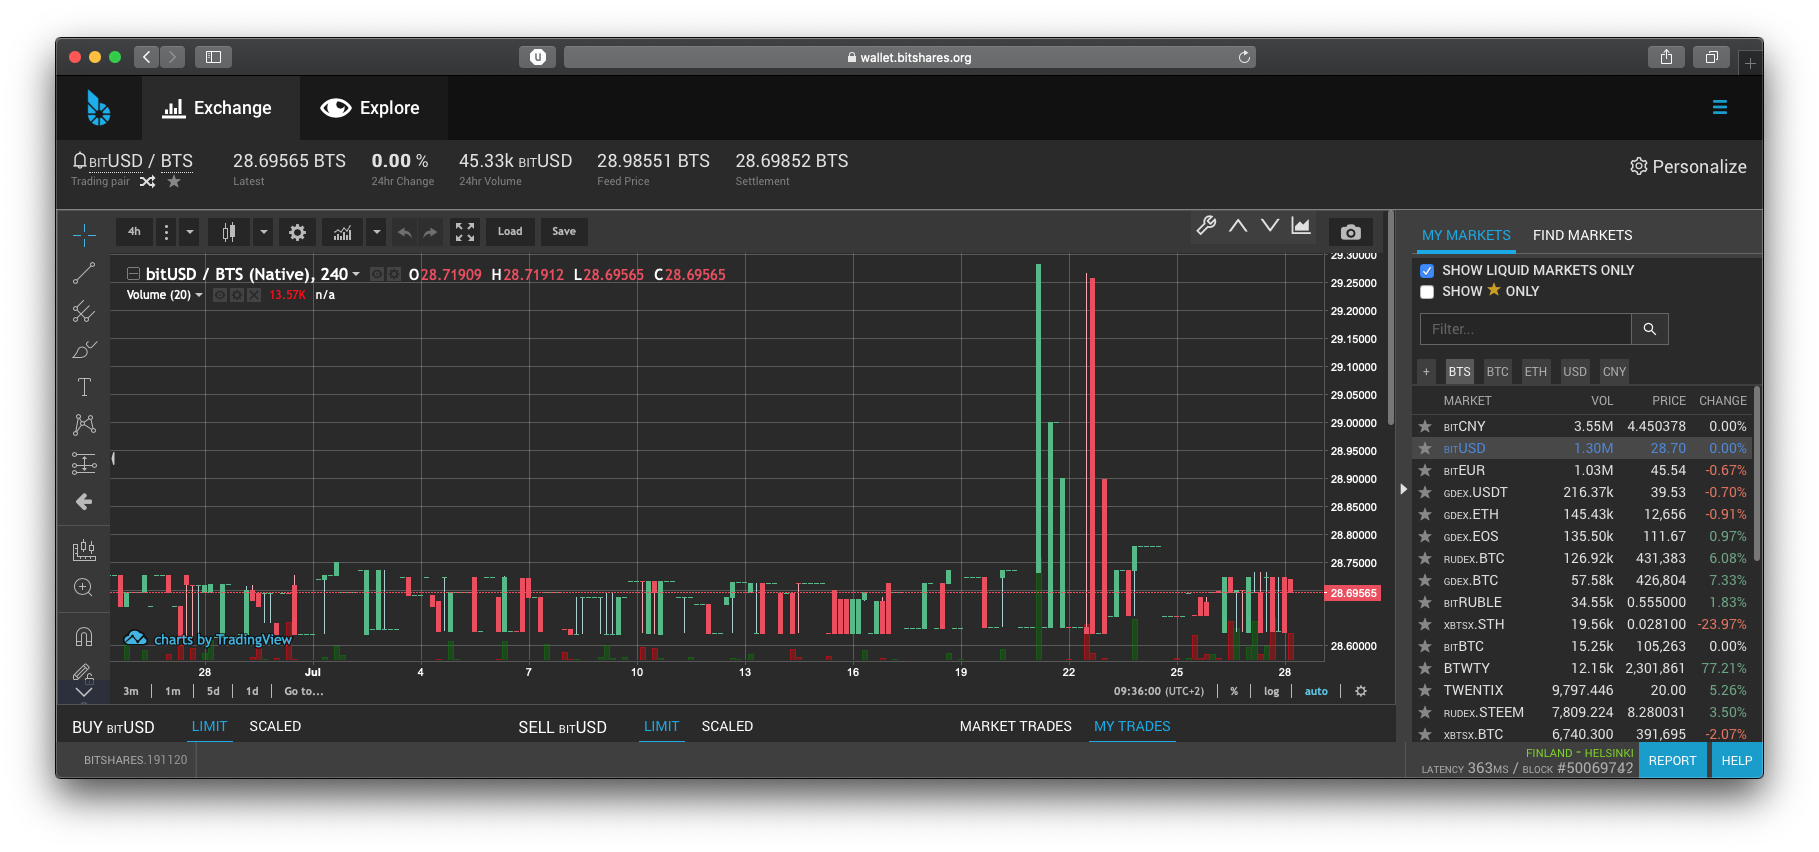
\includegraphics[width=\linewidth]{introduction/assets/bitshares}
	\caption{An online explorer provided by the BitShares DEX, showing recent and outstanding asset orders on the BitShares blockchain.}
	\label{fig:bitshares_explorer}
\end{figure}

\subsection{Blockchain-based Marketplaces}
The Bitcoin cryptocurrency and advancements in smart contract functionalities have demonstrated that it is possible for users to securely manage an ecosystem without trusted intermediaries.
After the success of Bitcoin, researchers and system developers started to explore how blockchain technology can replace key components of electronic marketplaces which are mostly operated by centralized providers~\cite{subramanian2017decentralized}.
We now outline how blockchain technology has been used to build new types of decentralized marketplaces, which we refer to as \emph{blockchain-based marketplaces}.

Beaver, introduced by Soska et al., is one of the earliest proposals that leverage blockchain technology to build an anonymous marketplace without trusted intermediary~\cite{soska2016beaver}.
Beaver uses a blockchain ledger to securely record user reviews and to store item listings while preserving privacy.
Beaver positions itself as a mechanism that is Sybil-resistant against fake vendor reviews, a key issue in \enquote{traditional} online marketplaces.
Beaver uses anonymous payment systems, e.g., Zerocash~\cite{sasson2014zerocash}, as platform currency.
The scalability of Beaver, however, is questionable since all data elements are stored on a distributed ledger secured by Proof-of-Work.

Blockchain technology is increasingly being used to build decentralized cryptocurrency exchanges, also called \emph{DEXes}.
DEXes enable the exchange of cryptocurrencies and other blockchain-based tokens without trusted intermediary.
A key advantage of DEXes is that users themselves remain in control of their funds and do not have to transfer ownership of their assets to the market operator.
The first generation of DEXes limits trading to assets residing on the same blockchain.
Notable examples include BitShares and Waves which have accumulated a market capitalization of X and Y dollars respectively.
On these markets, users can issue their own assets, transfer them to others, and trade these assets against other ones by publishing buy and sell orders on the blockchain.
Some DEXes provide an online interface with information on the outstanding orders and latest trades.
Figure~\ref{fig:bitshares_explorer} shows an online explorer of the BitShares blockchain, visualizing recent and outstanding asset orders.

\section{Disintermediation in Markets}
The popularity of electronic commerce has resulted in much interest to act as middlemen between buyers and sellers to benefit from their interactions~\cite{clark1999electronic}.
In many electronic markets, the role of matching buyers and sellers, and facilitating transactions is performed by a middlemen~\cite{bakos1998emerging}.
A well-known example is PayPal~\cite{paypal}, a payment service provider offering settlement services to customers buying goods from merchants.
PayPal not only process payments but it also acts as arbitrator when there a dispute between a buyer and seller arises.
The services of \emph{trusted intermediaries} such as PayPal is at the core of electronic market and ensures that a trade between a buyer and seller who might not necessarily trust each other proceeds without disputes.

Blockchain technology, and Bitcoin in particular, has challenged the need for trusted intermediaries.
In traditional payment systems, a financial institution acts as intermediary and handles payment between different (possibly foreign) banks.
Bitcoin has demonstrated that a decentralized system without financial institutions can be built, by leveraging cryptographic techniques.
Since the introduction of Bitcoin, there has been much effort by both industry and academia to critically look at the necessity of trusted intermediaries, and potentially replace them with another mechanism, e.g., smart contracts~\cite{lande2018sok}.
This process is also called \emph{disintermediation}.
Disintermediation usually lowers costs, since trusted intermediaries charge the involved traders for their services.
The process of disintermediation is tangential to the concept of decentralization (see Section X).
In particular, disintermediation requires decentralization as its foundation~\cite{guo2016blockchain}.

Disintermediation is a concept that pre-dates blockchain technology.
The Internet enabled quicker and convenient access to information, therefore opening opportunities to replace traditional broker agents~\cite{wigand2020whatever}.
A clear example of disintermediation can be found in the publishing market~\cite{giaglis1999disintermediation}.
Information technology enables book buyers to quickly place their order and authors to only print their books when there is actual demand.
This is also called printing-on-demand and removes the retailer from the traditional supply chain.

In many scenarios, it has been proven to be possible to disintermediate from a technical perspective.
Disintermediation is not always possible, nor desired.
However, in many scenarios there is a need to safeguard certain processes by intermediaries, in particular when considering the financial sector.
One might argue that electronic market require at least some intermediary to act as mediator between buyer and sellers if transactions are not atomic.
From a regulatory perspective, an intermediary can be required by law, e.g., when there is a need to verify the identify of new or existing business relations (this is also known as Know-your-Customer).

As also pointed out by other researchers, we argue that it is not likely that electronic markets will be fully disintermediated soon~\cite{zamani2018little}.
Rather than complete disintermediation, it is more likely that the role of existing intermediaries will be transformed.
For instance, financial institutions are currently exploring how distributed ledger technology can make their existing settlement services more efficient and reliable.
Perhaps the most influential solution, Corda, is currently being deployed by R3, a consortium consisting world's leading financial institutions~\cite{brown2016introducing}.
Another example is Ripple~\cite{armknecht2015ripple}, a credit network that is aimed to eventually replace the SWIFT payment infrastructure.
In practice, these solutions are not fully disintermediated since payments will still be processed by nodes operated by the involved financial institutions.


\section{Blockchain-based Marketplaces}
Given our definitions of decentralization and disintermediation in the context of electronic marketplaces, we now look how these concepts align with blockchain-based marketplaces.
Blockchain technology holds the promise to transform the market processes that currently require a trusted intermediary, e.g., when making payments to other peers.
It is important to clearly define what a blockchain-based marketplace means in the context of this work.
There is much confusion around the concept of blockchain-based marketplaces.
For example, the OpenBazaar market does not store its listings on a blockchain ledger but uses cryptocurrencies for peer-to-peer payments between merchants and customers.
In this work, \emph{a blockchain-based marketplace is a digital platform that leverages blockchain technology to carry out one or more of its critical operations}.

To better understand how this technology connects to existing market components, we describe the required components of blockchain-based marketplaces.
Figure~\ref{fig:electronic_markets} shows a decomposition of blockchain-based marketplaces.
This figure is the result of our literature survey where we have assessed both published and unpublished work on electronic marketplaces that use blockchain technology.
In general, we identify the following five mechanisms commonly used in blockchain-based marketplaces: \emph{matchmaking}, \emph{knowledge discovery}, \emph{settlement}, \emph{dispute resolution} and \emph{on-boarding}.
For each mechanism, we list approaches commonly found in the considered problem domain.
We now further discuss each identified mechanism. % the required components of blockchain-based marketplaces.

\begin{figure}[t]
	\centering
	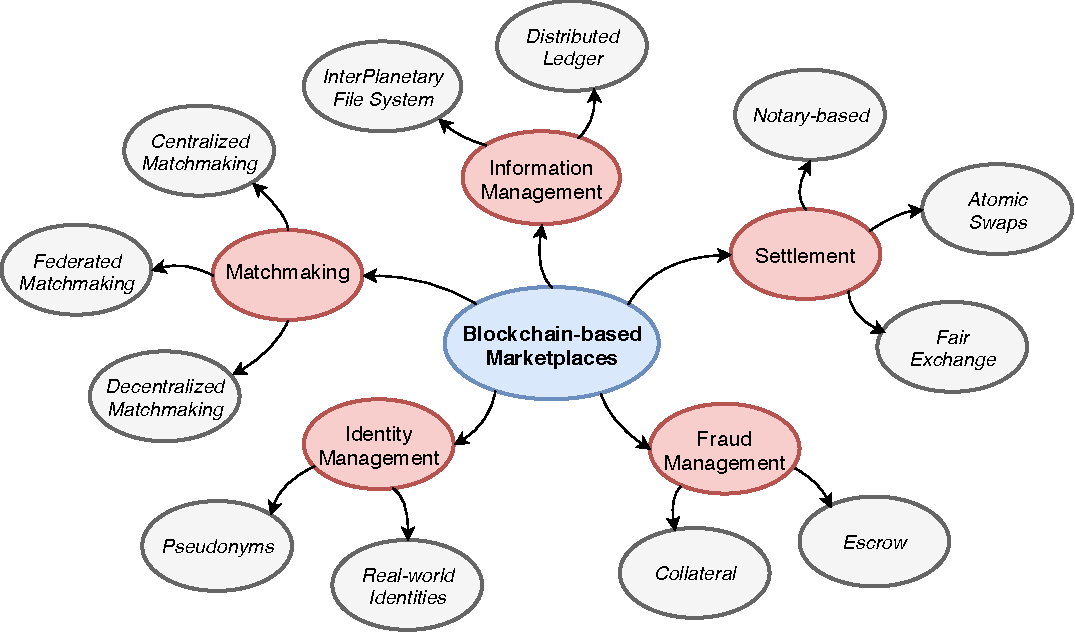
\includegraphics[width=\linewidth]{introduction/assets/decomposition}
	\caption{A decomposition of electronic marketplaces in four different components. Each component is further decomposed in approaches if applicable.}
	\label{fig:electronic_markets}
\end{figure}

\subsection{Knowledge Discovery}
Electronic marketplaces in general require a knowledge discovery mechanisms for market actors to enable value exchange.
Market knowledge includes pricing and product information, and details of past transactions.
Traditional electronic marketplaces usually store this information on centralized servers, deployed and managed by the market authority.
A key advantage of this approach for market operators is that these servers are relatively easy to setup and enable fast access to market information by participants.
Blockchain-based marketplaces usually avoid the storage of market information in a single location.
Therefore, market participants are dependent on others to retrieve the latest market state.

\subsubsection{Distributed Ledger}
A common approach for blockchain-based marketplaces is to store all available information on a distributed ledger.
This is, for example, the approach taken by DEXes like BitShares and Waves.
All market interactions are stored within tamper-proof transactions on a distributed ledger secured with global consensus.
Trades are either explicitly recorded in transactions, or can be derived from prior transactions.
Users wishing to get the latest market state are required to synchronize with the full distributed ledger from the network.
Since the distributed ledger might contain millions of transactions, some platform have setup a few \emph{full nodes} that remain synchronized in the network.
These full nodes offer an API that users can query to quickly retrieve market information.

\subsubsection{Order book}
A common market type is a financial exchange where financial instruments like currencies or bonds are being traded.
The buy and sell orders in these markets are usually bundled in an \emph{order book}.
An order book lists the specific assets or services that are being bought or sold within a market.
It provides traders with a convenient view on the current supply and demand.
Depending on the market and assets being traded, the order book sometimes reveals the identity of a trader behind an open order, or their reputation scores (for instance, Airbnb shows the reputation of hosts).
When presenting an order book to traders, ask and bid orders are usually sorted, i.e. based on their price.
For orders with a price, ask orders are sorted ascending on price in the order book and bid orders descending on price (the best orders are presented first).
%Market orders rarely end up in the order book as open order, since they are often fulfilled instantly.
%A defining metric used by traders is the difference between the price of the highest ask order and the price of the lowest bid order, also called the \emph{bid-ask spread}.
%For the order book shown in Figure \ref{fig:order_book}, the bid-ask spread is \$149.57 - \$149.54 = \$0.03.
%This metric also indicates market liquidity, the degree to which assets can be quickly bought or sold.
%A liquid market is often characterized by a low bid-ask spread.
The set of all ask or bid orders at a specific price is called a \emph{price level}.

\subsection{Settlement}
TODO

\subsubsection{Custodial}
A common approach to exchange blockchain-based assets is by using the services of a trusted intermediary.
A trade using a trusted intermediary completes as follows: two parties that agree on a trade transfer the assets for sale to one of the wallets owned by the trusted intermediary.
When this intermediary has received both assets, it finishes the exchange by transferring the appropriate assets to the other party.
In this approach, the trusted intermediary holds (temporary) ownership of the assets to be traded.
Relying on a trusted intermediary removes counterparty risk for the trading parties, but it requires both parties to have faith that the intermediary does not default or compromise their assets.

Trade through a trusted intermediary can facilitate value exchange between an extensive range of different blockchains, as long as the intermediary maintains wallets on the involved blockchains and can issue transactions in these systems to transfer the assets.
This is usually not an issue in permissionless blockchains since anyone can create accounts or wallets by generating a new cryptographic key pair.
Centralized cryptocurrency exchanges often facilitate asset trading across numerous permissionless blockchains.
Some cryptocurrency exchanges process transactions worth millions of dollars in total daily.\footnote{See https://coinmarketcap.com/rankings/exchanges}
In a permissioned blockchain environment, however, a trusted intermediary coordinating an asset exchange requires explicit approval from the operator to read and write transactions on the involved distributed ledgers.
Allowing new parties in a permissioned blockchain might be undesirable by operators since it introduces additional legal and operational risks.

\subsubsection{Atomic Swaps}
The \emph{atomic swap} is a distributed coordination task that allows asset exchange between different blockchains, without need for a trusted intermediary~\cite{herlihy2018atomic}.
Atomic swaps enable two parties to exchange blockchain-based assets with atomic guarantees: the asset exchange either completes or fails for both parties at any given time.
We now explain the involved operations during an atomic swap between the public Bitcoin and Ethereum blockchains.
Figure~\ref{fig:atomic_swap} visualizes the steps of an atomic swap between Alice and Bob, where Alice sells her Bitcoin in return for Ether (the native token of the Ethereum blockchain).
First, Alice generates a random secret $ s $ and computes $ H(s) $, where $ H(\cdot) $ denotes a hash function.
She then submits a hash-locked transaction, indicated by $ T_a(H(s)) $ (step \circled{1}), to the Bitcoin blockchain that transfers her Bitcoin to Bob's wallet address.
A hash-locked transaction is only executed when the secret $ s $ is provided to it.
Alice now sends $ H(s) $ to Bob (step \circled{2}).
Bob then submits a transaction $ T_b(H(s)) $ with the same hash lock to the Ethereum blockchain, transferring his Ethereum to the account of Alice (step \circled{3}).
Alice is now able to claim the assets held in custody by $ T_b(H(s)) $ (since she knows the value of $ s $), which in turn reveals $ s $ to Bob (step \circled{4}).
Bob now completes the swap by submitting $ s $ to the $ T_a(H(s)) $ transaction on the Bitcoin blockchain, which unlocks the assets in $ T_a(H(s)) $ (step \circled{5}).
To prevent the situation where assets are locked indefinitely if Alice refuses to reveal $ s $, Alice and Bob submit two additional time-locked transactions to ensure that assets in $ T_a(H(s)) $, respectively $ T_b(H(s)) $, can be claimed after some time $ t_1 $, respectively $ t_2 $.
To address the situation where Alice claims the assets in both $ T_a(H(s)) $ and $ T_b(H(s)) $, it must hold that $ t_1 > t_2 $.
These hash- and time-based agreements, also called Hashed Timelock Contracts (HTLCs), thus ensure trust-less, atomic asset exchange between trading parties, assuming that they claim the assets before the time-lock expires.
Atomic swaps eliminate the risk of losing assets to an adversarial trader while trading.
The HTLC atomic swap requires a total of four transactions.

\subsubsection{Notary-based}
Notary schemes are another solution for asset exchange where approval by a group of credible nodes (notaries) is required to perform some operation.
Notary schemes aim to partially alleviate the trust issues arising when relying on a single trusted intermediary through the approval by a group of semi-trusted notaries instead.
These notaries reach consensus on the occurrence of particular events, e.g., on the inclusion of a transaction on a distributed ledger.
Compared to an asset exchange through a trusted intermediary, notary schemes assume a weaker trust model and can often withstand adversarial behavior of a fraction of the notaries.

The Interledger project, introduced by Ripple, is the most advanced approach in this direction~\cite{thomas2015protocol}.
Interledger proposes a notary-based protocol to conduct payments across different ledgers.
In atomic mode, these payments are realized through atomic swaps and are coordinated by a different group of notaries for every involved blockchain.
Interledger uses payment paths where additional intermediate platforms and their notaries are used to exchange assets between ledgers that do not have a direct connection.
Interledger also supports bidirectional asset exchange but is vulnerable to a fraction of notaries colluding with one of the trading parties.
External coordination is avoided in universal mode, which relies on incentives for participants to behave honestly and not to commit fraud.
The Hyperledger Quilt project provides a Java implementation of the Interledger protocol for permissioned blockchains~\cite{hyperledgerquilt}.

\subsubsection{Fair Exchange}
TODO

\begin{figure*}[t]
	\centering
	\begin{subfigure}[t]{.33\textwidth}
		\centering
		\captionsetup{width=.9\linewidth}
		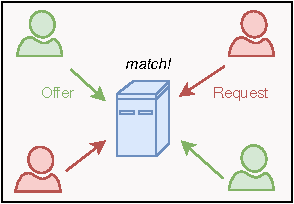
\includegraphics[width=.9\linewidth]{introduction/assets/centralized_matchmaking}
		\caption{\emph{Centralized matchmaking}: new orders are always sent to a single matchmaker, usually a centralized system (server).}
		\label{fig:centralized_matchmaking}
	\end{subfigure}%
	\begin{subfigure}[t]{.33\textwidth}
		\centering
		\captionsetup{width=.9\linewidth}
		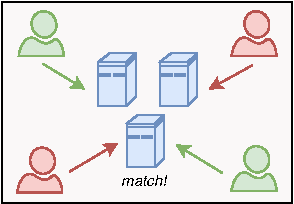
\includegraphics[width=.9\linewidth]{introduction/assets/federated_matchmaking}
		\caption{\emph{Federated matchmaking}: new orders are sent to one of the available matchmakers in the network.}
		\label{fig:federated_matchmaking}
	\end{subfigure}%
	\begin{subfigure}[t]{.33\textwidth}
		\centering
		\captionsetup{width=.9\linewidth}
		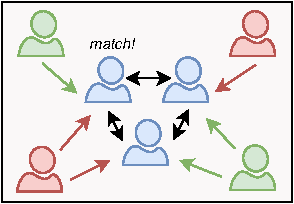
\includegraphics[width=.9\linewidth]{introduction/assets/decentralized_matchmaking}
		\caption{\emph{Decentralized matchmaking} (our proposal): new orders are sent to multiple matchmakers and shared between them.}
		\label{fig:decentralized_matchmaking}
	\end{subfigure}
	\caption{Three models for order matching. Traders create offers and requests (colored green and red respectively), which are matched by matchmakers (depicted in blue).}
	\label{fig:matching_models}
\end{figure*}

\subsection{Order Matchmaking}
\label{sec:matchmaking}
Automatically \emph{matching} customers is a prerequisite for online trade and therefore essential for electronic marketplaces.
Matchmaking is defined as the process of mediating supply and demand in markets, based on profile information~\cite{Veit:2003fs}\footnote{In multi-agent systems, a matchmaker is considered as an entity that only aggregates offers. Brokers aggregate both offers and requests. We will use the term matchmaker in this paper since we found it to be more common in related work.}.
Notable examples are matching idle agents to incoming jobs or matching suppliers of specific assets to consumers who are interested in buying these assets.
Inefficient matchmaking between participants decreases overall market efficiency and customer satisfaction~\cite{Wu2015TheM}.
%For example, in a ride-hailing marketplace like Uber, it is key to match nearby drivers and passengers in a timely and efficient manner.
For instance, prolonged suboptimal matching by ride-hailing marketplaces such as Uber increases the waiting time for passengers and results in drivers having to traverse a greater distance to pick up their customers.
%Similarly, inefficient matching of available computer resources to customers by cloud providers could violate service-level agreements, resulting in customer loss and reputational damage.

In this section, we review different approaches to order matchmaking in electronic markets.
Matchmaking depends on the individual constraints and preferences of market participants.
In most electronic markets, a participant includes this information in an \emph{order} that indicates their intention to buy and sell assets, resources, or services~\cite{Veit:2003fs}.
This order is then submitted to a matchmaker.
In general, economic literature distinguishes between two types of orders: \emph{asks}, created by traders offering a specific asset, service, or resource, and \emph{bids}, created by interested buyers.
%Each order can have multiple attributes attached, e.g., a price or a location.
The main objective of a matchmaker is a quick and effective mediation between incoming offers and requests, based on constraints and preferences included in each order.

We identify three different approaches to order matchmaking, depicted in Figure~\ref{fig:matching_models}.
With \emph{centralized matchmaking} (Figure~\ref{fig:centralized_matchmaking}), traders submit their asks and bids to a single server.
With \emph{federated matchmaking} (Figure~\ref{fig:federated_matchmaking}), traders submit a new order to one of the servers of their choice.
Finally, in \emph{decentralized matchmaking} (Figure~\ref{fig:decentralized_matchmaking}), traders submit their orders to one or more matchmakers.
We further elaborate on each matchmaking model.

\subsubsection{Centralized Matchmaking}
Figure~\ref{fig:centralized_matchmaking} visualizes the centralized matchmaking model, which is the most common approach to match orders.
Traders send new offers and requests to a dedicated matchmaker, usually a centralized system (server).
This model is widely adopted by commercialized marketplaces such as stock exchanges or peer-to-peer service markets like Uber.
A matchmaker bundles open orders in a local data structure known as an \emph{order book}.
The order book stores all active asks and bids, and provide traders a convenient view on the current supply and demand.
A new incoming ask or bid is then matched with other bids and asks, respectively, using a \emph{matching policy}.
The most common matching policy used in cryptocurrency exchanges is the \emph{price-time} strategy, where orders are first matched based on the price, and then on their order creation time (older orders are prioritized).
The order book is often optimized for fast order lookup and matching within a specific trading domain.

The EtherDelta decentralized exchange is one of the first DEXes that adopt the centralized matchmaking model~\cite{Anonymous:brZbAflS}.
EtherDelta maintains a single server that stores an order book with all active orders.
Traders can browse the order book and trade against orders in the order book.
The trades are finalized on the blockchain, and the order is then removed from the EtherDelta order book.\todo{custodial vs non-custodial}
The IDEX exchange also deploys a centralized server but automatically matches orders submitted by makers and takers~\cite{AuroraLabs:B4jmyRY8}.
Specifically, traders lock their assets in the IDEX smart contract and submit their order to the IDEX server, which checks its validity.
The order is then executed by the Ethereum smart contract and the order book is updated according to the executed trade.

A main advantage is that the centralized matchmaking model with a single server is relatively straightforward to implement, since no communication or order book synchronization is required.
Also, since all orders are stored and matched by single matchmaker, orders are processed based on full market knowledge.
The identity behind each order is only known to the market operator, therefore protecting the privacy of individual traders.

Unfortunately, the emergence of electronic trading in general gave rise to fairness, transparency and manipulation issues during the matchmaking process~\cite{Mavroudis:2019iw}.
For example, the EtherDelta operator is able to censor specific orders.
Furthermore, information asymmetry between exchange operators and traders allows operators to front-run specific orders (see Section X\todo{x}).
The work of Mavroudis and Melton address fairness issues arising from the latency traders experience when submitting orders and gaining market information~\cite{Mavroudis:2019iw}.
They propose Libra, an order reordering matching policy that alleviates the effects of uneven delays by the market infrastructure.
Libra remains temporally fair, meaning that among all pairs of participants on it the probability that a slower participant succeeds in capturing a trading opportunity at the expense of a faster participant (who, responsive to the same stimulus, is also competing for the same opportunity) does not exceed 0.5.

From a systems perspective, centralized matchmaking has a low scalability compared to distributed solutions since the matchmaker becomes a bottleneck when more orders are created in the same time period.
Fault tolerance is another concern: if the single matchmaker becomes unavailable, e.g., due to infrastructure failures, incoming orders cannot be matched and all market activity stalls.

\subsubsection{Federated Matchmaking}
Figure \ref{fig:federated_matchmaking} illustrates an alternative model for order matching: federated matchmaking.
Instead of relying on a central matchmaker, multiple (independent) matchmakers individually maintain an order book.
The group of matchmakers can either be static (e.g., elected by a committee or a voting mechanism), or dynamic (e.g., each peer can opt-in to become a matchmaker).
A trader now submits new orders to their preferred matchmaker (for example, based on the reliability or trustworthiness of individual matchmakers).
The 0x and Swap protocols are notable examples of the federated matchmaking model and are discussed next.

%Blockchain-powered marketplaces based on the 0x and AirSwap protocols have adopted the federated matchmaking model~\cite{warren20170x}~\cite{oved2017swap}.
The 0x protocol uses off-chain order relaying and on-chain settlement, meaning that orders are created shared, and matched outside a blockchain.
A maker creates market liquidity in 0x by first selecting an available relayer.
Each relayer maintains an off-chain order book and charges a transaction fee for its services.
The maker then creates the order and specifies a fee which is given by the selected relayer.
Takers query the order book of relayers and if they intend to fulfill an order, they submit it to the Ethereum blockchain.
The Augur prediction market (see Section~\ref{sec:prediction_markets}) leverages the 0x protocol for order dissemination and matching.

The Swap protocol follows a similar off-chain matchmaking, on-chain settlement model~\cite{oved2017swap}.
In Swap, indexers aggregate trade intents created by market makers and takers.
The indexer informs takers when a matching trade intent has been found, upon which a peer-to-peer negotiation process starts between the matched maker and taker.
During this negotation process, a maker may contact an oracle to get a price suggestion.
When a maker and taker agree on a trade, the taker submits the agreement to an Ethereum smart contract, upon which the trade is executed and on-chain assets are exchanged.
We remark that both 0x and Swap are limited to trading Ethereum-based digital tokens and can therefore not be used for order processing of any blockchain-based asset.

The federated matchmaking model gives traders the opportunity to use the services of their preferred matchmaker.
Manipulative behaviour of one matchmaker then leads to the situation where traders select another, honest matchmaker.
Furthermore, unavailability of an individual matchmaker is less likely to stall all market activity since a trader can send their orders to another available matchmaker.
However, the order book is fragmented across different matchmakers, potentially leading to less market efficiency and liquidity, compared to matchmaking with an order book managed by a single entity.

\subsubsection{Decentralized Matchmaking}
%Scalability limitations, low fault tolerance, and uneven load balancing are inherent issues of centralized and federated matchmaking.
The \emph{decentralized matchmaking} model is depicted in Figure \ref{fig:decentralized_matchmaking}.
The main idea is that a single order is sent to multiple matchmakers simultaneously and matchmakers share their orders with other matchmakers (liquidity sharing).
We distinguish between on-chain and off-chain decentralized matchmaking.

\textbf{On-chain.}
We now discuss on-chain matchmaking approaches that either rely on a smart contract to match incoming orders, or embed the matchmaking logic in the transaction validation logic.
The Stellar protocol integrates DEX functionality that enables users to create buy and sell orders that trade assets native to the Stellar ledger~\cite{Lokhava:2019kd}.
These orders are created using specific transaction types, that are matched with existing, outstanding orders during inclusion of the transaction in the ledger.
The Stellar matching engine uses the price-time policy.
Similarly, the BitShares blockchain provides functionality to create orders at the protocol level~\cite{Schuh:CsvWDxUZ}.

The main advantage of on-chain matchmaking is tight integration with the blockchain platform; no external components such as a peer-to-peer overlay are needed to process orders.
Instead, all orders can simply be processed by the blockchain logic.
This also makes it more convenient for users to submit their orders.
On the other hand, since users likely need to pay transaction fees when creating new orders or when cancelling existing ones, trading in bulk can become a costly process.
Furthermore, blockchain-based order matching can be orders of magnitude slower compared to centralized matchmaking, due to security requirements.
Finally, on-chain matching protocols do not explicitly store the history of matches.
Therefore, the reconstruct the order book at a specific block height, one needs to process all transactions up to that point.

\textbf{Off-chain.}
To overcome transaction fees and slow transaction confirmation times, some platforms maintain a fully decentralized order book off-chain.
An example of off-chain decentralized matchmaking is the Loopring protocol, which builds a decentralized order sharing protocol~\cite{Wang:wt}.
Loopring is able to mix and match multiple orders in circular trade, also called order rings, therefore increasing liquidity.
New orders are sent to one or more relays in a mesh network.
Order rings are submitted to a smart contract, e.g., on Ethereum, where the trade is then executed.
Relayers can optionally share orders with other relayers to increase liquidity, however, the whitepaper lacks technical details on how this is achieved specifically.
Relayers take the margin between two matched orders, or can charge some fee.
% front-running in Loopring

The Republic Protocol builds a decentralized network of nodes that match orders without revealing any information about individual orders~\cite{Zhang:kGvi0me4}.
Specifically, it uses Shamir Secret Sharing to break down an order in multiple order fragments which are distributed through the network.
An Ethereum smart contract, called the Registrar, describes the network topology such that it is hard for an adversary to fully reconstruct an original order.
Nodes cooperate with other nodes to check if their order fragments match, by computing a zero-knowledge proof.
When two order fragment match, an atomic swap is initiated between the two traders (also see Section~\ref{sec:atomic_swap}).
Note that this prevents an individual from estimating the total liquidity in the network.

We identify two advantages of this model over centralized and federated matchmaking.
First, sharing orders between matchmakers can yield the same matching effectiveness compared to centralized matchmaking, depending on the order synchronization details. %since orders can be synchronized amongst matchmakers.
Second, decentralized matchmaking should show higher tolerance against failure of individual matchmakers.
However, this model increases bandwidth usage since orders are sent to multiple matchmakers.
Also, it might take longer before a new order is fulfilled in the case that it is sent to matchmakers that are unable to match this order immediately.

\subsection{Identity Management}
Identity management is a key component of any electronic market.
Traditional electronic marketplaces usually impose some form of identity validation before a user is allowed to engage in trade with other users.
In this situation, the digital identity is linked to real-world credentials, e.g., a passport.
Identity validation in electronic marketplaces has several purposes.
First, it adds accountability of ones actions within the market in case of a dispute between a buyer and seller.
Second, it prevents the situation where a user can easily re-enter the market under a different identity after having committed fraud.
Third, identity verification is often part of the regulatory compliance of market operators, as often required by anti-money laundering policies.
Most cryptocurrency exchanges managed by a central market authority require users to verify their identity before they can create buy or sell orders.

In stark contrast with traditional marketplaces, a key property of blockchain technology is the ability to join the network under a pseudonym, using a locally generated cryptological keypair.
In Bitcoin, for example, users can easily transfer Bitcoin to others using different digital identities.
This is even the preferred practice when one wants to retain anonymity in the Bitcoin network.
Similarly, many DEXes do not require identity verifications and allow traders to join the network under a pseudonym.

\subsection{Fraud Management}
Fraud is a key concern in electronic marketplaces.
A common type of fraud is \emph{counterparty fraud}, where a party does not fulfil its obligation towards the counterparty during trade settlement, e.g., by not delivering the promised assets or goods.
This kind of fraud is often resolved by the market operator, acting as arbitrator during the dispute resolution process.
Within blockchain-based marketplaces, counterparty fraud is often prevented since asset exchange is atomic: either all parties receive their assets or nothing happens.
This approach works when assets can be exchanged directly, e.g., on a blockchain-powered DEX.
Fraud management, however, is required when settlement depends on the actions by users.
We identify different approaches to manage fraud.

\subsubsection{Escrows}
TODO

\subsubsection{Collateral}
Some blockchain-based marketplaces require users to deposit collateral before trading.
This collateral is slashed when its depositor does not adhere to an agreement and therefore incentivise traders to follow the protocol.
The XClaim protocol relies on collateral deposits to enable asset trading between distinct blockchain ledgers.
When a participant deviates from the protocol, the collateral is slashed and wronged actors are reimbursed.

%\section{Problem Statement}
%The key issue is that decentralized applications that are using blockchain technology are often not scalable enough.

\section{Research Questions}
In this thesis, we mainly focus on \emph{knowledge discovery}, \emph{matchmaking} and \emph{settlement} in electronic markets.

The overarching research question of this thesis is as follows:\\\\
\emph{How can we improve matchmaking and settlement mechanisms in blockchain-based marketplaces?}\\\\
To answer our research question, we address the following key questions:

\textbf{[RQ1] What is the state-of-the-art in blockchain-based electronic trading and asset exchange?}
To provide an answer to our research question, it is required to build an understanding of state-of-the-art approaches to blockchain-based trading, and their shortcomings.
Even though there is much active research on blockchain-based decentralized exchanges and secure asset trading between heterogeneous blockchain platforms, the field lacks a systematic literature overview, an analysis of open challenges and suggestions for further research.

\textbf{[RQ2] How can we efficiently match market orders without centralized coordinator?}
The predominant approach to order matchmaking in electronic markets is by using a centralized server, owned by the market operator.
This approach, however, enables manipulation by the operator, resulting in an unfair system.
Blockchain-based matchmaking has the potential to address fairness issues but is by far not scalable enough for usage by many marketplaces.
We aim for an efficient matchmaking mechanism with fairness guarantees, not under the control of a single market operator.

\textbf{[RQ3] How can improve settlement durations of (international) payment infrastructures?}
A major problem of current banking systems is that the settlement duration of a payment between two different (international) banks is significant, often in the order of days.
Furthermore, these payments require significant transaction fees to cover back-office costs.
Blockchain technology holds the potential to improve the speed of (international) payment infrastructures, and potentially lead to a reduction of costs and lower transaction fees.

\textbf{[RQ4] How can we exchange assets managed by different blockchains?}
Decentralized exchanges (DEXes) is a new type of decentralized application where digital assets are issued and traded on a blockchain.
Compared to centralized exchanges, DEXes take a non-custodial approach where users manage these assets themselves.
The main issue, however, is that the assets on a specific DEX are locked to a single blockchain; trade between different DEXes is either impossible or slow.
The question is how to address these issues and enable fast asset trading between different exchanges.

\textbf{[RQ5] How can we apply blockchain technology to improve software crowdsourcing markets?}
The engineering of blockchain-based applications such as exchanges is a challenging task and requires engineers with appropriate qualifications.
Crowdsourcing is a relatively new model for software development, where an open call is made for the documentation, design, coding, and testing of software.
Recent research proposes to leverage blockchain technology
Applying accountability and fraud detection could improve the software crowdsourcing process.

\begin{table*}[t]
	\small
	\centering
	\begin{tabular}{ |c|c|c|c| }
		\hline
		\textbf{Chapter} & \textbf{Mechanism} & \textbf{DAS5 experiments?} & \textbf{Deployment?} \\ \hline
		2 & TrustChain & yes & yes, integration in Tribler \\ \hline
		3 & MATCH & yes & yes, integration in Tribler \\ \hline
		4 & XChange & yes & yes, integration in Tribler \\ \hline
		5 & Internet-of-Money & yes & in-house testing \\ \hline
		6 & DevID & no & user trial \\ \hline
	\end{tabular}
	\caption{An overview of research methods for each mechanism introduced in this thesis.}
	\label{table:research_methodology}
\end{table*}

\section{Research and Engineering Methodology}
Blockchain technology is a relatively new and immature field.
We identify two fundamentally different approaches to the adopted research methodology in this field.
On one hand, published blockchain research in systems-oriented conferences follow an experimental methodology where the performance of the proposed mechanism is systematically evaluated using a comprehensive set of experiments and benchmarks.
On the other hand, there is a vast body of research on the security aspects of distributed ledgers.
This kind of research tend to follow a more theoretical approach through the use of formal proofs or small-scale protocol simulations.

In this work, we adopt an experimental-driven approach where we answer each research question by designing, implementing and evaluating a system or mechanism.
We then systematically evaluate the appropriate properties of each mechanism, and if feasible, we deploy our mechanisms to users to gather real-world results.
For all of our proposed mechanisms, we aspire a practical solution, ready for deployment and usable by real users.

Distributed systems can be complex software implementations with many components that work together.
Specifying the scope of a system is a non-trivial challenge and failing to implement clear system boundaries can result in numerous performance bottlenecks and degradation of user experience when such a system is deployed.
To this end, during the design of each mechanism we specify the boundaries of each system and state what we consider out of scope.
We aim to focus on the core functionality of each mechanism.

Table~\ref{table:research_methodology} specifies for each mechanism whether we present a set of DAS5 experiments and/or whether we have conducted a real-world deployment.
Except for DevID, we evaluate each component using a comprehensive set of experiments that have been conducted on our DAS5 nation-wide compute cluster.

Driven by our focus on practicality, we have deployed each mechanism proposed in this thesis, either to a small group of users or with an integration in Tribler.
Tribler is our academic testbed and offers decentralized, anonymous file-sharing capabilities.
Tribler has been downloaded by over 1.5 million users and enables us to test our ideas in a geo-distributed, real-world environment.
We have evaluated TrustChain, for example, in the context of our anonymous file-sharing overlay to address free-riding behaviour.
This longitudinal deployment allowed us to incrementally improve our software and refine our ideas.
Due to legal considerations, we have been unable to provide an open-source implementation of the Internet-of-Money mechanism.

We ensure that each mechanism is tested.
Even though this is uncommon practice for research projects, we believe that a proper engineering methodology adds credibility to the presented mechanisms, helps reproducibility and is instrumental in getting a system ready for deployment.

% simplicity?

%We believe this experimental research methodology is suitable for two reasons.
%First, it allows us to evaluate our ideas in an environment that closely resembles a real-world environment.
%Second, it directly leads to a software implementation that can be used by academia or industry.
%All developed software artefacts are available on our GitHub repository and contain unit tests to verify functional correctness.

% existing research does X

% but we do Y!

\begin{figure}[t]
	\centering
	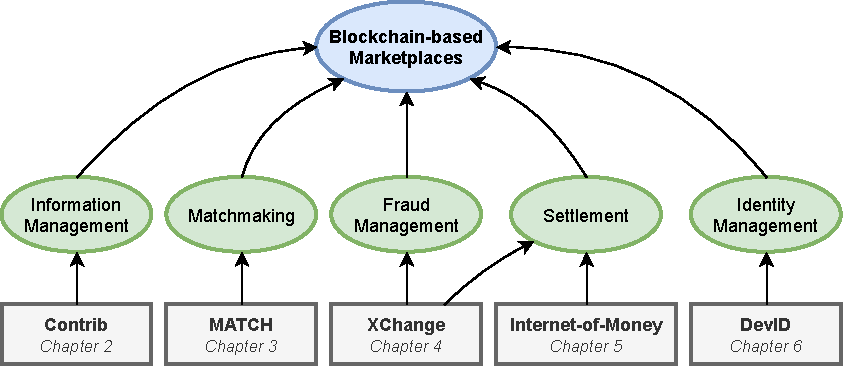
\includegraphics[width=\linewidth]{introduction/assets/thesis_overview}
	\caption{The five mechanisms presented in this work (depicted in grey), in the context of blockchain-based marketplaces and their components.}
	\label{fig:thesis_overview}
\end{figure}

\section{Contributions and Thesis Outline}
After establishing the required background on decentralized applications and distributed ledger technology, Chapter \todo{X} highlights scalability limitations of state-of-the-art blockchain ledgers.
Next, in Chapter \todo{X}, we design, implement and evaluate TrustChain: a scalable blockchain ledger that is based on fraud \emph{detection} instead of fraud \emph{prevention}.
In Chapters \todo{X to Y}, we apply accountability primitives and fraud detection techniques in three well-established domains: financial transactions, two-sided marketplaces, and identity.
Specifically, we make the following contributions in each chapter:\\

\textbf{[Chapter 2] SoK: Electronic Markets in the Age of Blockchain.} (Work in progress)
In this chapter, we answer RQ2 and provide an extensive overview of existing approaches for online trade in the age of blockchain.\\

\todo{Work in progress}\\

\textbf{[Chapter 3] MATCH: Accountable and Generic Matchmaking for Decentralized Applications.}
In this chapter, we partially address RQ4 and focus on matchmaking, the process of bringing market participants together based on individual preferences.
Matchmaking is a cardinal, yet overlooked prerequisite for a fully decentralized exchange.
Although numerous companies have deployed infrastructure for matchmaking, there is currently no solution that can be deployed within different trading domains.
We present MATCH, a middleware for generic order matching.
Since MATCH is agnostic about order specifications, the resulting system is highly flexible and reusable.
In this work, we first present an alternative approach to order matching, named \emph{decentralized matchmaking}.
The main idea is that new orders are disseminated to multiple matchmakers simultaneously and shared between matchmakers.
We then design and implement a novel matching protocol and a middleware with full support for both existing matchmaking paradigms and decentralized matchmaking.
Finally, we extensively evaluate desired system properties of MATCH under a real-world ride-hailing and asset trading workload.
Our main finding is that decentralized matchmaking exhibits superior fault tolerance and load balancing, at the cost of moderately increased bandwidth usage and order completion time.
This chapter is based on the following publication:

\todo{UNDER REVIEW}\\

\textbf{[Chapter 4] XChange: A Scalable Asset Marketplace based on Accountability.}
In this chapter, we answer RQ4 and introduce XChange, an asset marketplace based on accountability guarantees.
There is an increasing need for a generic mechanism to trade assets across isolated platforms, as more industries rely on the digital management of their physical resources using Internet-of-Things devices.
To date, there is no such mechanism without dependency on a trusted third party.
We address this shortcoming and present XChange, a blockchain-based mechanism for generic asset trading.
Unlike existing asset trading marketplaces, we decouple trade management and the actual exchange of assets.
XChange enables the trustworthy trade of \emph{any} digital asset.
We describe a generic trading protocol that establishes trade between individuals and accounts market activity on any distributed ledger.
We prove with a theoretical analysis that the effectiveness of fraud conducted by adversarial parties is limited.
Furthermore, we devise a novel market architecture, composed of all required components for a decentralized asset marketplace.
We implement the XChange mechanism and conduct real-world evaluations.
To account market activity in a tamper-proof manner, we use an existing scalable blockchain ledger, TrustChain.
By deploying XChange on multiple low-resource devices, we show that a full trade can be completed within 500 milliseconds.
To analyze the scalability and bandwidth usage, we conduct further experiments on our compute cluster and deploy up to 500 XChange instances.
Our main finding is that the throughput of XChange, in terms of trades per second, scales linearly with the network size.
This chapter is based on the following publication:

\todo{UNDER REVIEW}\\

\textbf{[Chapter 5] Internet-of-Money: Applying Accountability to Enable Real-time International Money Transfers.}
In this chapter, we answer RQ3 and explore a new stage in the evolution of digital trust, trusting strangers with your money.
We address the challenging problem of giving money to others and relying on them to forward it.
To identity fraud, we account money transfers between interacting strangers.
This work represents a small step towards a generic infrastructure for trust, moving beyond proven, single-vendor platforms like eBay, Uber and AirBnb.
Expanding upon trust relations, we designed, implemented and evaluated an overlay network: \emph{Internet-of-Money}.
Internet-of-Money is capable of real-time money transfers to different banks by routing funds through individuals (\emph{money routers}).
This removes the need for central banks to handle a payment.
Our network reduces traditional payment durations from a day or even a few days in weekends, to mere seconds.
%Internet-of-Money is fully decentralized, privacy-preserving and highly scalable.
With real-world experimentations, we prove that Internet-of-Money enables fast money forwarding.
We show that our overlay network is capable of discovering a majority of available money routers within a minute.
Finally, we demonstrate how profit of cheating routers is limited and that misbehaviour is punished.
This chapter is based on the following publication:

Martijn de Vos and Johan Pouwelse, \enquote{Real-time Money Routing by Trusting Strangers with your Funds}, \emph{IFIP Networking, 2018.}\\

\textbf{[Chapter 6] DevID: Blockchain-based Portfolios for Software Developers.}
In this chapter, we answer RQ5.
Decentralized applications, also known as dApps, are the new paradigm for writing business-critical software.
Recruiting developers with appropriate qualifications and skills for this activity is key, yet challenging.
The main problem is that the portfolio of developers is usually scattered across centralized platforms like GitHub and LinkedIn, and vendor locked.
This can result in an incomplete impression of their capabilities.
We address this problem and introduce \emph{DevID}, a blockchain-based portfolio for developers.
Over time, this portfolio enables developers to build up a trustworthy collection of records that showcase their capabilities and expertise.
They can import data assets from third parties into a unified DevID portfolio, add projects and skills, and receive endorsements.
All portfolio records are stored on a scalable distributed ledger and owned by developers themselves.
The essential idea is to exploit the tamper-proof property of the blockchain while providing durable storage.
To demonstrate the practical value of DevID, we build the competition-based platform, \emph{dAppCoder}, for the development of decentralized applications.
On dAppCoder clients are able to submit their ideas and developers can find work.
dAppCoder utilizes DevID portfolios to match these clients and developers.
We fully implement our ideas and conduct a deployment trial.
Our trial demonstrates that DevID is efficient at storing portfolio records.
This chapter is based on the following publication:

Martijn de Vos, Mitchell Olsthoorn and Johan Pouwelse, \enquote{DevID: Blockchain-based Portfolios for Software Developers}, \emph{IEEE International Conference on Decentralized Applications and Infrastructures (DAPPCON'19)}\\

\textbf{[Chapter 7] Conclusion.} We will end this thesis with the conclusion, a summary of the lessons learned, and suggestions for further work.

%\begin{figure}[t]
%	\centering
%	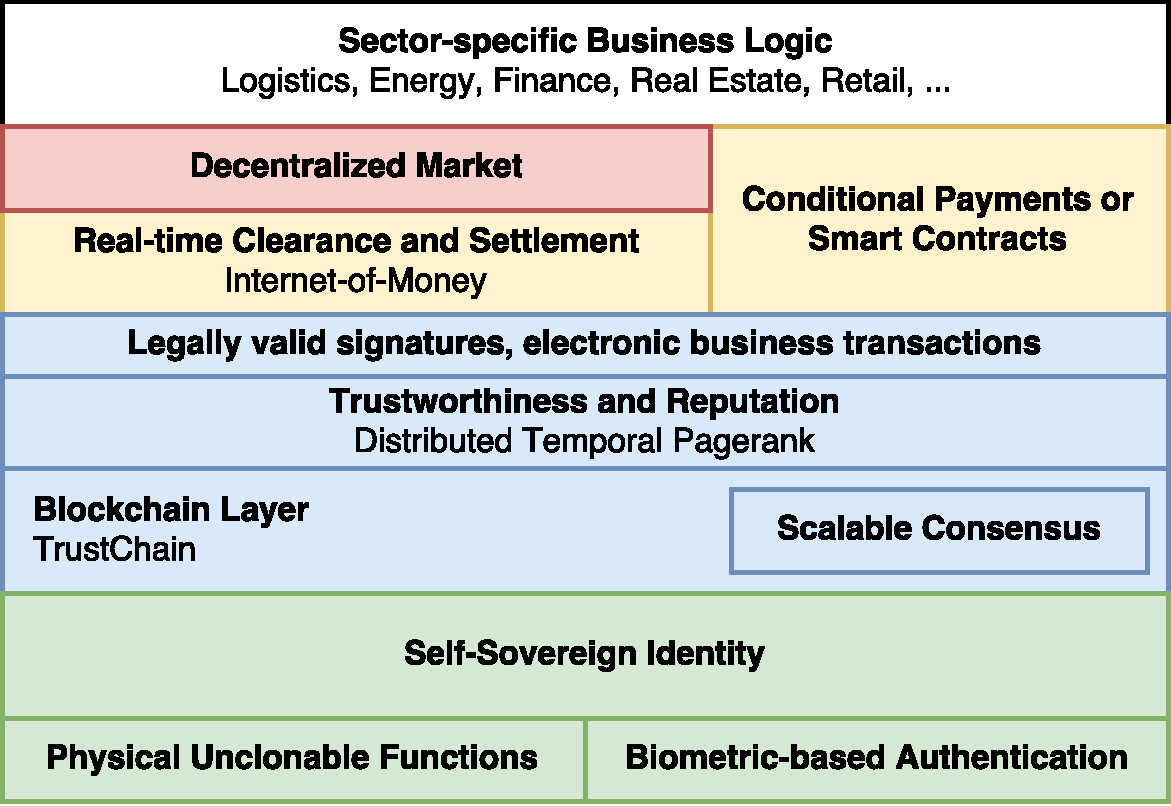
\includegraphics[width=.7\linewidth]{introduction/assets/tech_stack}
%	\caption{An overview of the research conducted at the Delft Blockchain Lab.}
%	\label{fig:dbl_tech_stack}
%\end{figure}

%\section{About the Delft Blockchain Lab}
%The Delft Blockchain lab is Delft's initiative for research, education and training in blockchain technology and trust on the Internet.
%Figure~\ref{fig:dbl_tech_stack} outlines the research directions of the Delft Blockchain Lab, ranging from low-level primitives like biometric-based authentication to sector-specific business logic.
%At the lowest layers (depicted in green), we build, deploy and evaluate new solutions for managing ones identity in the physical world and on the Internet.
%These solutions include biometric-based authentication and physical unclonable functions, a method to securely store a private key.
%A part of our ongoing research includes a self-sovereign identity solution that is currently being tested and deployed in the Netherlands.

%Our research effort around distributed ledger technology includes scalable consensus algorithms and Sybil-resistant reputation mechanisms.
%The TrustChain distributed ledger is presented in Chapter X.
%The other components of this thesis are mostly focussed on the research directions that are coloured yellow and red in Figure~\ref{fig:dbl_tech_stack}.
%For a detailed outline of our research efforts, we refer the reader to our published vision paper.

%\newpage

%\bibliographystyle{unsrt}
%\bibliography{introduction}